% fig_mechanism_shapes.tex -- creative/explanatory: a clean, standalone
% redraw of "which response shape is it" (same geometry as Fig.~1 panel c,
% but bigger, on its own, with each of the THREE shapes drawn separately
% so a reader can absorb one at a time rather than overlaid). Good for the
% Metrics or Problem section as a companion to Eq.~(pri)/(cbi).
% Draft only, not wired into main.tex.

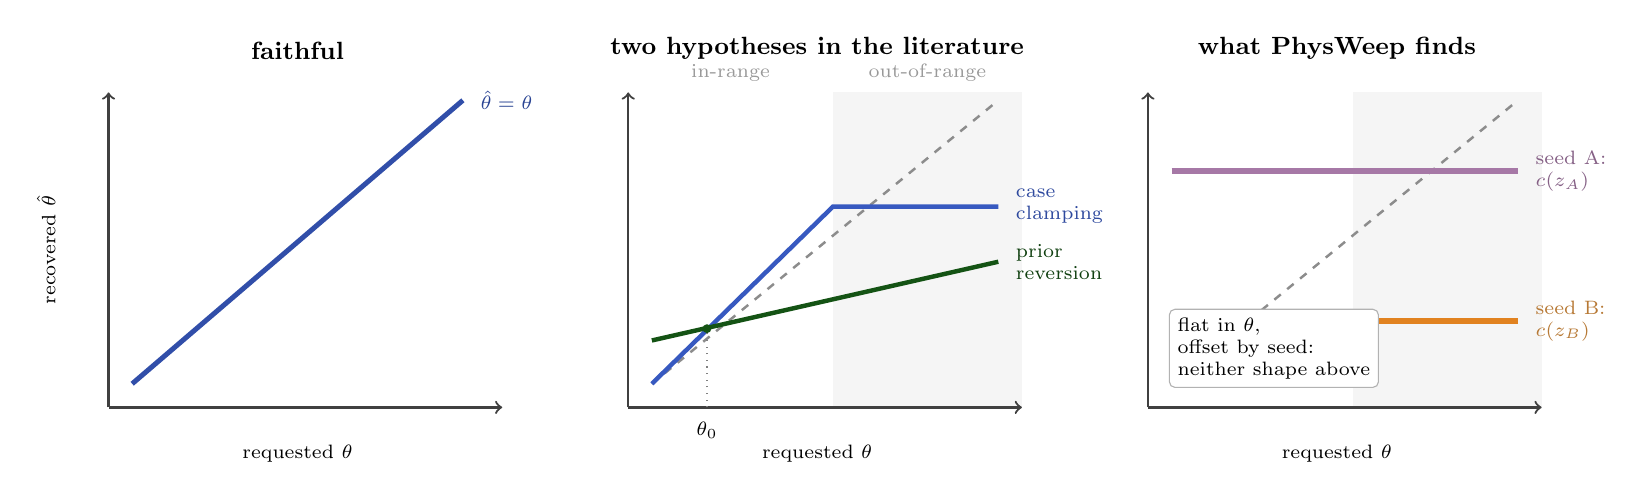
\begin{tikzpicture}[
  font=\small,
  ax/.style={->,thick,black!75},
  ideal/.style={dashed,black!45,line width=0.9pt},
  panelbg/.style={fill=black!4},
]

% ---------- PANEL 1: faithful ----------
\begin{scope}
  \node[anchor=south,font=\bfseries\small] at (2.4,4.3) {faithful};
  \draw[ax] (0,0) -- (5.0,0);
  \draw[ax] (0,0) -- (0,4.0);
  \node[font=\scriptsize,anchor=north] at (2.4,-0.35) {requested $\theta$};
  \node[font=\scriptsize,rotate=90,anchor=south] at (-0.55,2.0) {recovered $\hat\theta$};
  \draw[RoyalBlue!75!black,line width=1.8pt] (0.3,0.3) -- (4.5,3.9);
  \node[RoyalBlue!65!black,font=\scriptsize,anchor=west] at (4.6,3.9) {$\hat\theta=\theta$};
\end{scope}

% ---------- PANEL 2: the two prior hypotheses ----------
\begin{scope}[shift={(6.6,0)}]
  \node[anchor=south,font=\bfseries\small] at (2.4,4.3) {two hypotheses in the literature};
  \fill[panelbg] (2.6,0) rectangle (5.0,4.0);
  \draw[ax] (0,0) -- (5.0,0);
  \draw[ax] (0,0) -- (0,4.0);
  \node[black!40,font=\scriptsize,anchor=south] at (1.3,4.02) {in-range};
  \node[black!40,font=\scriptsize,anchor=south] at (3.8,4.02) {out-of-range};
  \node[font=\scriptsize,anchor=north] at (2.4,-0.35) {requested $\theta$};
  \draw[ideal] (0.3,0.3) -- (4.7,3.9);
  % case clamping: follows identity then flat
  \draw[RoyalBlue!85!black,line width=1.6pt] (0.3,0.3) -- (2.6,2.55) -- (4.7,2.55);
  \node[RoyalBlue!70!black,font=\scriptsize,anchor=west,align=left] at (4.8,2.55)
    {case\\clamping};
  % prior reversion: shallow line crossing identity at theta_0
  \draw[ForestGreen!60!black,line width=1.6pt] (0.3,0.85) -- (4.7,1.85);
  \fill[ForestGreen!60!black] (1.0,1.0) circle (1.6pt);
  \node[ForestGreen!45!black,font=\scriptsize,anchor=west,align=left] at (4.8,1.85)
    {prior\\reversion};
  \node[font=\scriptsize,anchor=north] at (1.0,-0.06) {$\theta_0$};
  \draw[black!50,dotted] (1.0,0) -- (1.0,1.0);
\end{scope}

% ---------- PANEL 3: what we actually find ----------
\begin{scope}[shift={(13.2,0)}]
  \node[anchor=south,font=\bfseries\small] at (2.4,4.3) {what PhysWeep finds};
  \fill[panelbg] (2.6,0) rectangle (5.0,4.0);
  \draw[ax] (0,0) -- (5.0,0);
  \draw[ax] (0,0) -- (0,4.0);
  \node[font=\scriptsize,anchor=north] at (2.4,-0.35) {requested $\theta$};
  \draw[ideal] (0.3,0.3) -- (4.7,3.9);
  % two flat, seed-conditional levels
  \draw[Plum!75!black,line width=2.0pt] (0.3,3.0) -- (4.7,3.0);
  \draw[BurntOrange!90!black,line width=2.0pt] (0.3,1.1) -- (4.7,1.1);
  \node[Plum!60!black,font=\scriptsize,anchor=west,align=left] at (4.8,3.0)
    {seed A:\\$c(z_A)$};
  \node[BurntOrange!70!black,font=\scriptsize,anchor=west,align=left] at (4.8,1.1)
    {seed B:\\$c(z_B)$};
  \node[draw=black!30,fill=white,rounded corners=2pt,inner sep=3pt,
        font=\scriptsize,align=left] at (1.6,0.75)
    {flat in $\theta$,\\offset by seed:\\neither shape above};
\end{scope}

\end{tikzpicture}
